%! Author = melek
%! Date = 22.01.2023

% Preamble
\documentclass[11pt]{article}

% Packages
\usepackage{amsmath}
\usepackage{graphicx}
\graphicspath{ {../images/} }

\title{Assignment 4: Model Based RL}
\author{huseyinabanox@gmail.com}
\date{January 2023}

% Document
\begin{document}

    \maketitle

    \section*{Problem 1}

    \subsection*{First Run}

    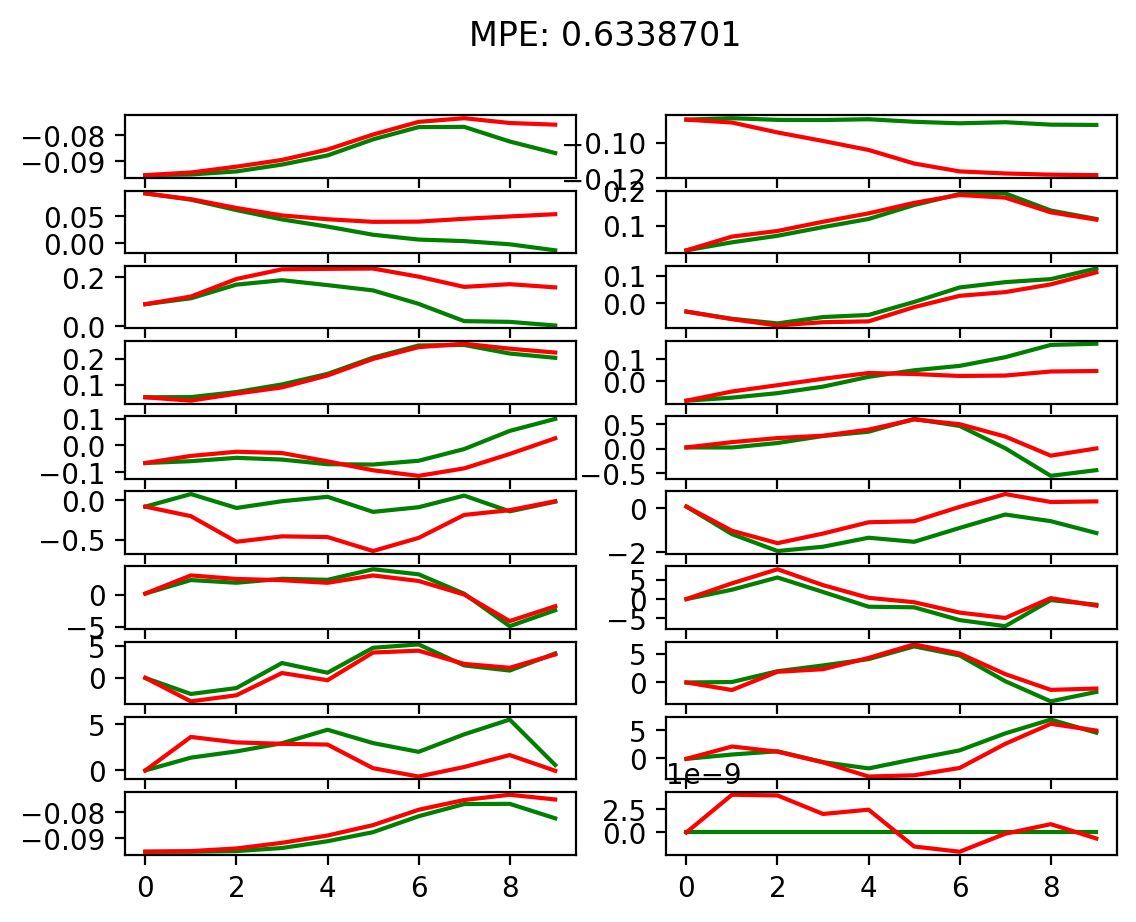
\includegraphics[scale=0.9]{q1/itr_0_predictions_run0}

    A small network is used.
    Results can be improved using a larger network.

    \subsection*{Second Run}

    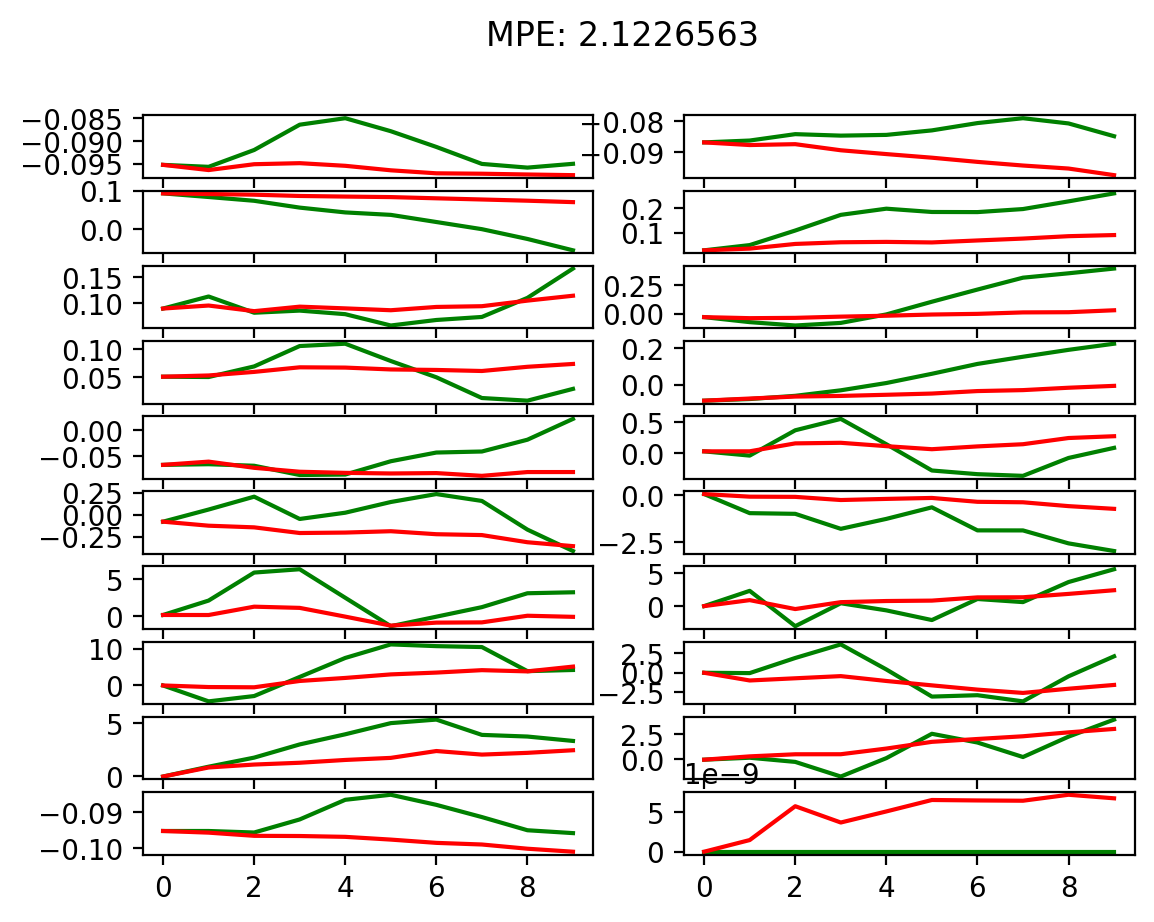
\includegraphics[scale=0.9]{q1/itr_0_predictions_run1}

    Small number of iterations are used.
    Results can be improved by increasing iteration count.
    MPE is the worst.

    \subsection*{Third Run}

    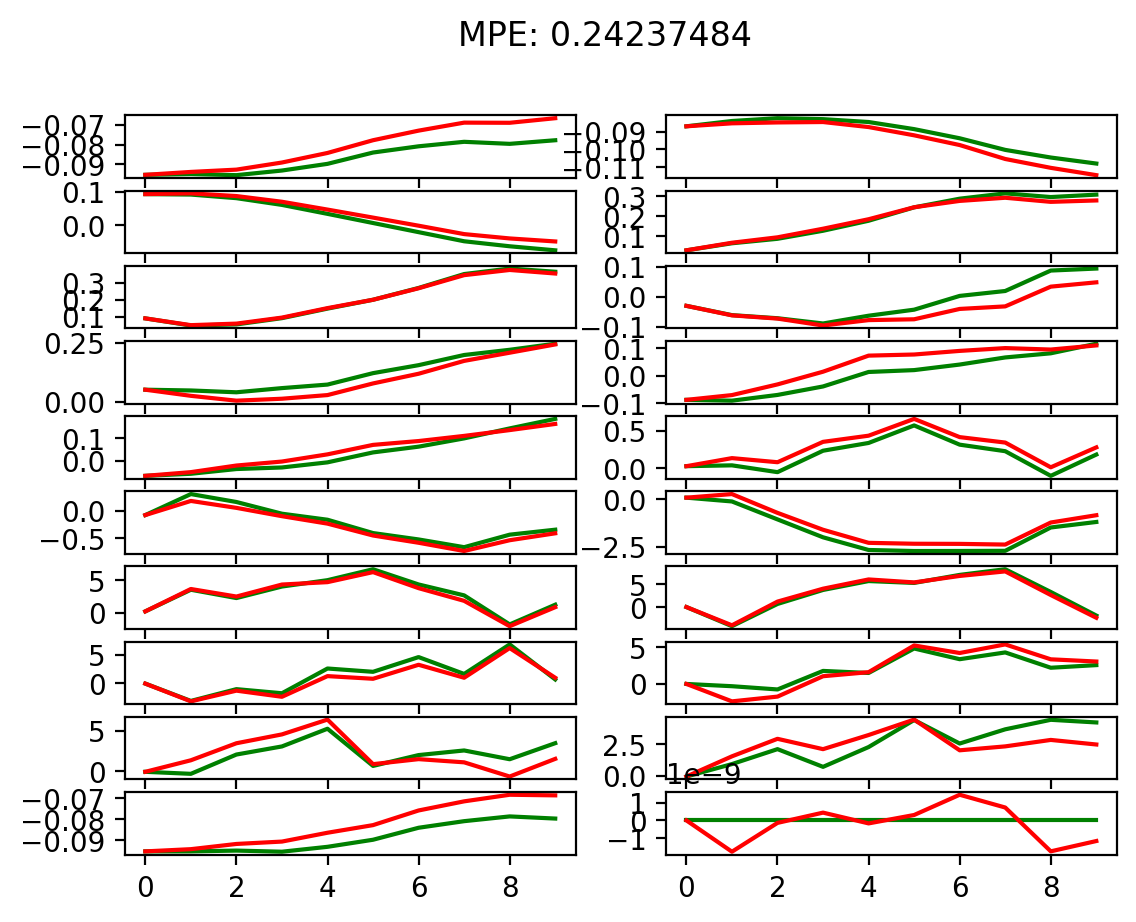
\includegraphics[scale=0.9]{q1/itr_0_predictions_run2}

    Best results are obtained using a larger network and more iterations.
    MPE is the best.

    \section*{Problem 2}

    Train AverageReturn is expected to be around -160 and Eval AverageReturn is expected to be around -70 to -50.

    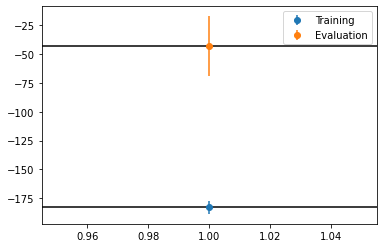
\includegraphics[scale=0.9]{q2/q2}

    Actual returns are around the expected values.

    \section*{Problem 3}

    MBRL algorithm with on-policy data collection and iterative model training.
    Rl trainer.py already aggregates your collected data into a replay buffer.
    Thus, iterative training means to just train on our growing replay buffer while collecting new data at each iteration using the most newly trained model.

    \hspace*{-0.6in}
    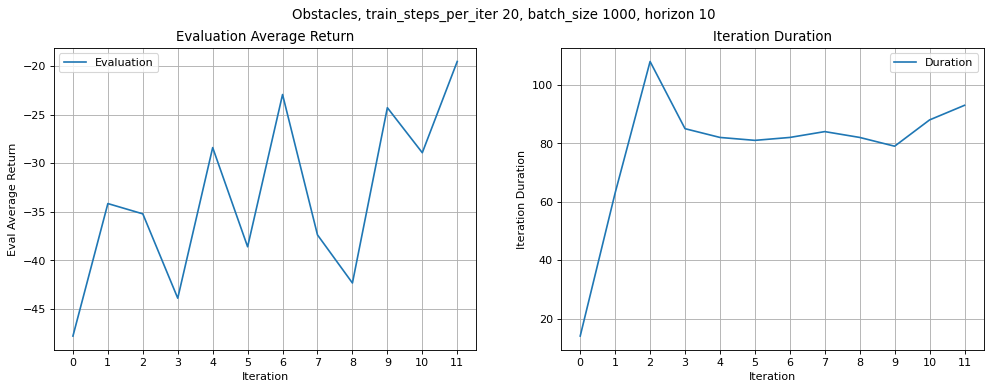
\includegraphics[scale=0.5]{q3/obstacles}

    Rewards of around -25 to -20 is expected for the obstacles env.
    The actual results are similar.

    \hspace*{-0.6in}
    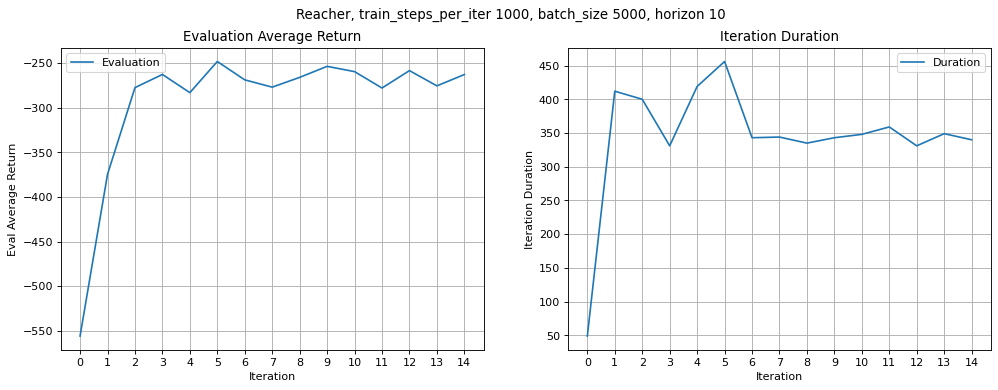
\includegraphics[scale=0.5]{q3/reacher}

    Rewards of around -250 to -300 is expected for the reacher env.
    The actual results are similar.

    \hspace*{-0.6in}
    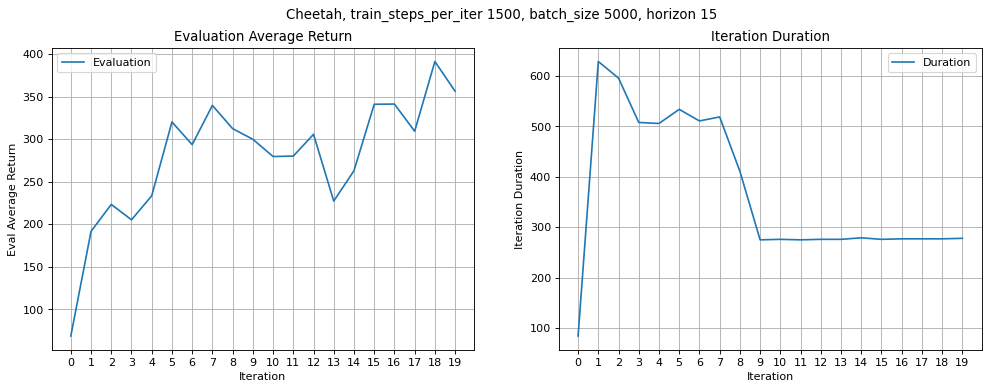
\includegraphics[scale=0.5]{q3/cheetah}

    Rewards of around 250 to 350 is expected for the cheetah env.
    The actual results are similar.

    \section*{Problem 4}

    \hspace*{-0.6in}
    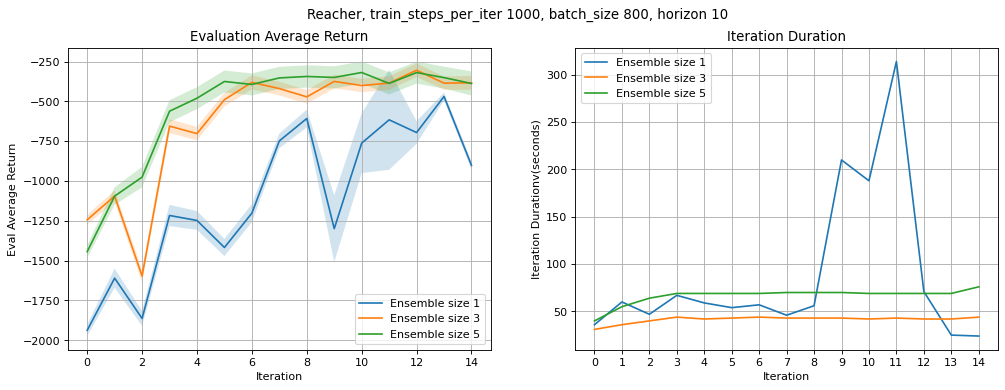
\includegraphics[scale=0.5]{q4/networks}

    The chart above shows effect of ensemble size.
    Increasing ensemble size improves average return but at the cost of training time.
    Intermediate values proposes the best trade off.

    \hspace*{-0.6in}
    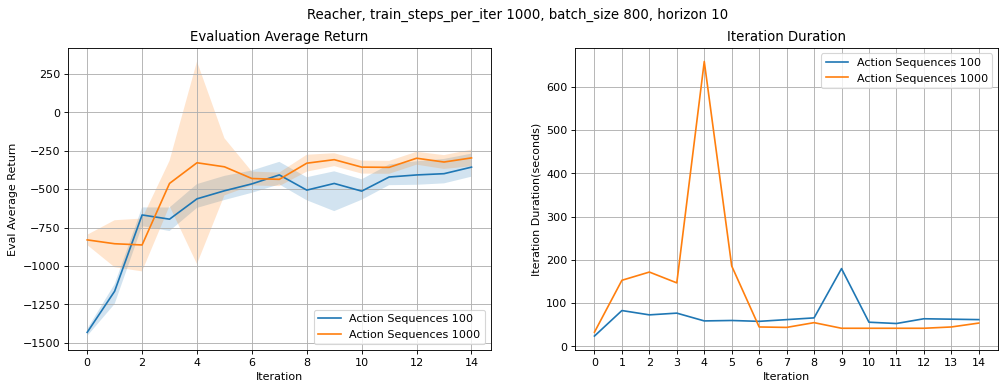
\includegraphics[scale=0.5]{q4/actions}

    Increasing action sequence count improved average return slightly.
    Training time increases as well but the chart shows a mixed view.
    A more reliable duration chart should incorporate average of multiple runs.

    \hspace*{-0.6in}
    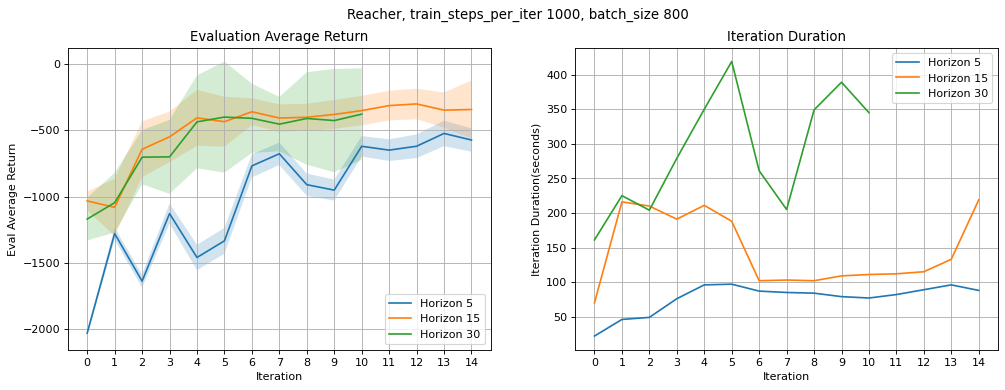
\includegraphics[scale=0.5]{q4/horizon}

    Increasing action horizon improves average return but also increases variance.
    The final difference is not too much.
    The most apparent effect increasing the horizon is seems to be increasing the training speed.
    Again the value is obtained using the intermediate values.

    \section*{Problem 5}

    \hspace*{-0.6in}
    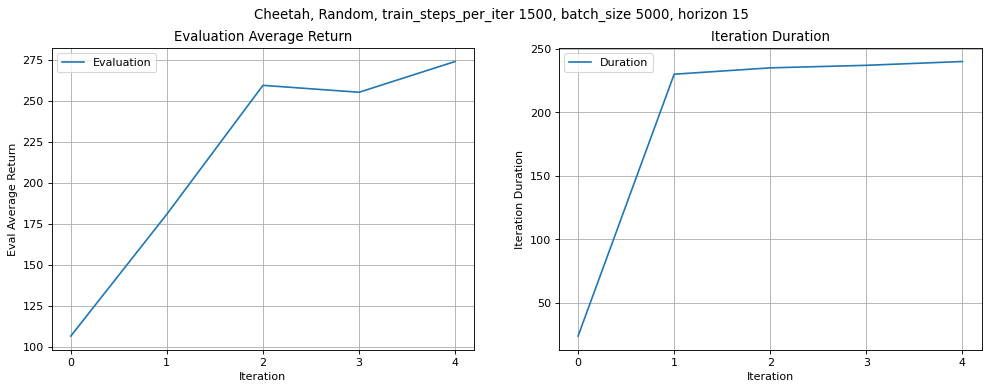
\includegraphics[scale=0.5]{q5/random}

    \hspace*{-0.6in}
    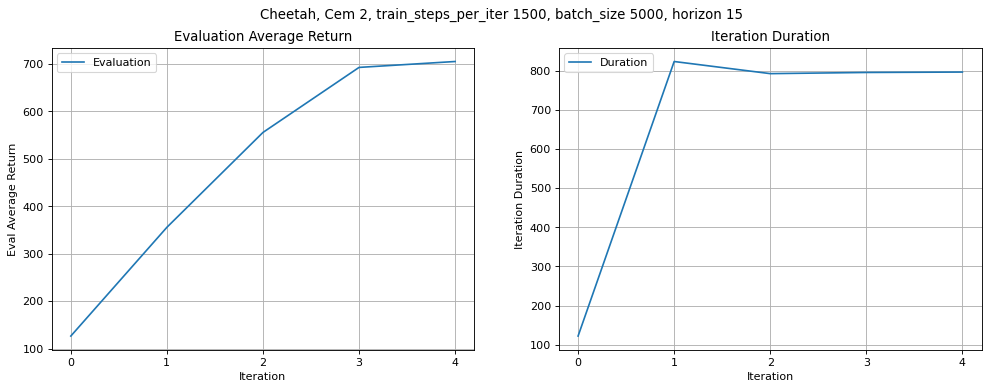
\includegraphics[scale=0.5]{q5/cem2}

    \hspace*{-0.6in}
    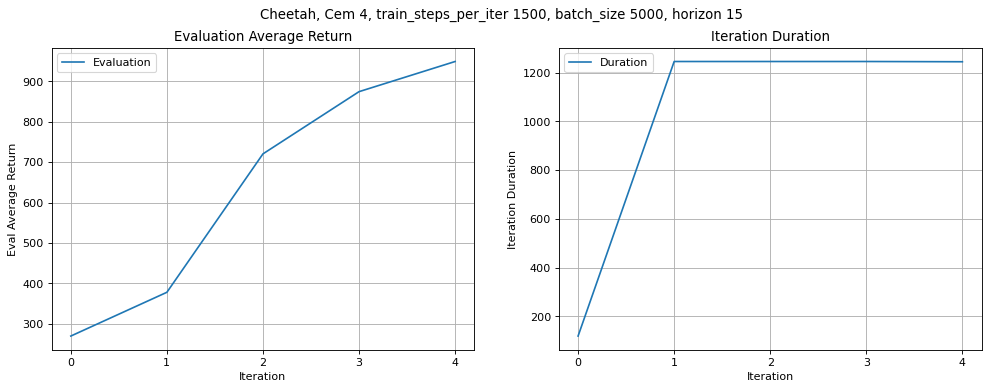
\includegraphics[scale=0.5]{q5/cem4}

    The charts show the effect of using cem.
    Using cem has a clear advantage over random sampling.
    Iteration duration increases similarly.
    4 iteration cem yields better return at the cost of dramatically longer iterations.
    2 iteration cem provides better value by providing a better return/duration ratio.

\end{document}